\documentclass[english,twoside, openright, hidelinks, 11 pt, class=report,crop=false]{standalone}
\input{../bm}
\input{../../preamb}


\begin{document}
\section[Oppgaver med tall og situasjoner fra virkeligheten]{Oppgaver med tall og situasjoner fra virkelig-heten}	
\st{Se også oppgaver på \net{https://ektedata.uib.no/}{ekte.data.uib.no}}


\subsection*{Oppgaver for grunnskole og P-fagene}
\op{opggaafart}
Vanlig gåfart regnes for å være ca. 1,5\enh{m/s}. Hvor langt kommer man med denne farten
\abc{
	\item etter 25 min?
	\item etter 3 timer?
}	
	
\op{opgtorden}
\tagop{
	\#overslag \#proporsjonalitet
}
Når det er lyn og torden kan du bruke følgende metode for å finne ut omtrent hvor langt unna du er uværet:\os

\st{Start med å telle sekunder straks du ser et lyn. Stopp tellingen når du hører torden. Gang antall sekunder med 300, da har du et overslag på hvor mange meter du er unna uværet.}

Bruk internett til undersøke hastigheten til lys (lyn) og lyd (torden) i luft, og forklar hva denne metoden baserer seg på.
\newpage
\op{opgstigningsgrad}
\tagop{
\#prosent \#negative tall \#tekstforståelse
}
Statens vegvesen definerer \outl{stigningsgrad} slik:
\st{
Stigningsgrad er definert som høydeforskjell dividert med horisontal avstand i vegens lengderetning.
Stigningsgraden uttrykkes vanligvis i \%. Den er positiv i stigning og negativ i fall sett i
profileringsretningen.
}
Ved starten av bratte veistrekker bruker det å stå skilt som varsler om veiens stigningsgrad. \os

Si at stigningen på et veistrekke starter 2 meter over havet, og slutter 10 meter over havet, og at veistrekket er 100 meter i horisontal retning. 
\abc{
\item Hva er stigningsgraden til dette veistrekket?
\item Hva menes med at stigningsgraden er ''negativ i fall sett i\\ profileringsretningen''?
}

\op{opgstorlstar} 
\tagop{
	\# modellering \# areal
}
Gitt et rektangel med omkrets 4, og la $ x $ være den éne sidelengden.
\abc{
	\item  Finn uttrykket til funksjonen $ A(x) $, som viser aralet til rektangelet.
	\item Hva er $ x $ når rektangelet har størst areal? Hvilken form har rektangelet da?
}
\mers{I \refops{opgstorlstar2} finner du en \textit{generalisert} utgave av denne oppgaven. Med andre ord kan det vises at formen du finner i oppgave b) alltid vil være den formen et rektangel må ha for å ha et størst mulig areal i forhold til omkretsen.}

\newpage
\op{opgprogprim}
\tagop{\#programmering \#primtall}
Skriv et skript som lykkes i å finne alle primtall på intervallet\\ 1-100.

\op{opglysar}
\tagop{	\# omgjøring av enheter \# standardform \# proporsjonale størrelser }
Lysets hastighet i vakuum er tilnærmet lik $ 3\cdot10^8\enh{km/s} $.
\abc{
\item Et \outl{lysår} angir distansen et objekt vil reise hvis det beveger seg med lysets hastighet i ett år. Hvor langt er et lysår?
\item Lys bruker ca. 8 minutt på å bevege seg fra Sola til Jorda. Hvor langt er det mellom Sola og Jorda?
}


\op{opgdusj}
\tagop{
	\# omgjøring av enheter \# standardform \# proporsjonale størrelser 
}
Det har blitt populært å regne ut hva det koster å ta seg en dusj. Til et slikt reknestykke kan man gjøre følgende antakelser:
\begin{itemize}
	\item Energien som kreves er energien som må til for å varme opp vannet som gikk med til dusjingen fra 7$^\circ $ til $ 35^\circ $.
	\item For å øke temperaturen til 1 liter vann med 1$ ^\circ $, kreves det $ 4,2\cdot10^3\enh{J} $.
\end{itemize}
Ifølge \net{https://www.vg.no/spesial/2022/stromprisene/}{vg.no} er 645,26 øre/kWh den høyeste (gjennomsnittlige) strømprisen registrert i Oslo. 
\abc{
	\item Regn ut hva en dusj på 10 minutter ville kostet med denne prisen. 
	\item Bruk internett til å finne strømprisene for din region i dag. Sjekk hva en 10 minutters dusj vil koste deg.
}
\textit{\small Obs! I denne oppgaven ser vi bort ifra \outl{nettleie}. Alle strømforbrukere må betale nettleie for frakt av strøm, og jo mer strøm man forbruker, jo høyere vil nettleien være, men strømprisen vil ha mest å si for hvor mye en dusj koster.}
\newpage
\op{opgtannhjul}
\tagop{
	\#faktorisering \#primtall
}
I et system hvor to tannhjul virker sammen, er det ønskelig at en tann og et kammer møtes så sjeldent som mulig. Dette for å unngå slitasje. \vsk

\abc{
	\item Et tannhjul med 12 tenner er koblet til et tannhjul med 21 tenner, som vist i figuren under. Hvor mange omdreininger må det røde tannhjulet ta for at tann A og kammer 1 skal møtes igjen?
	\item Gjenta spørsmålet fra oppgave a), men hvor det blå tannhjulet er erstattet med et tannhjul som har 11 tenner?\footnote{Legg merke til at antall tenner og antall kammer alltid vil være like}.
	\item Hvis to tall ikke har noen annen felles faktor enn 1, sier vi at de er \outl{relativt primiske}. Hvorfor er systemer med tannhjul helst innrettet slik at antall tenner på de forskjellige tannhjulene er relativt primiske?
}
\fig{tannhjul}
\newpage
\linje
Hvis en størrelse har veldig høy verdi, kan det være lettere å \\forestille seg omfanget til størrelsen ved å sammenligne den med en konkret størrelse (i motsetning til å bruke SI-enhetene gram, meter og lignende). Oppgave \ref{opgbluewhale} - \ref{opgregnskog} handler om slike sammenligninger.\\
\linje

\op{opgbluewhale}
\tagop{\#enheter \#regning \#}
Ifølge \net{https://www.wwf.no/dyreleksikon/bl\%C3\%A5hval}{WWF} kan en blåhval veie opp til 200\enh{tonn}, og ifølge \net{https://www.geno.no/om-geno/om-norsk-rodt-fe/karakteristikk-hos-nrf/}{geno.no} kan en norsk NRF-ku veie opp til 650\enh{kg}. Hvor mange NRF-kyr tilsvarer vekten av én blåhval?

\op{opgamazonas}
\tagop{
	\#proporsjonale størrelser \#volum \#overslag
}
\outl{Vannføringen} i en elv viser til volumet vann en elv frakter per tidsenhet. I en \net{https://en.wikipedia.org/wiki/List_of_rivers_by_discharge}{Wikipedia}-artikkel om verdens største elver kan man lese følgende:\regv

\st{
	(...) The average flow rate at the mouth of the Amazon is sufficient to fill more than 83 such pools each second.\vsk
	
	\textsl{\textbf{Norsk oversettelse}\\ (...) Den gjennomsnittlige vannføringen i munningen av Amazonas-elven er nok til å fylle mer enn 83 slike per sekund.}
}

Gjengi utregningene som er brukt for å finne de to tallene i teksten over, når du vet at artikkelen har brukt følgende som utgangspunkt:
\begin{itemize}
	\item Bassenget det er snakk om er et olympisk svømmebasseng, som har har lengde 50\enh{m}, bredde 25\enh{m} og dybde 2\enh{m}.
	\item Den gjennomsnittlige vannføringen i Amazonas-elven er 209\,000\enh{m}$ ^3 $/\text{s}.
\end{itemize}
\newpage
\op{opgregnskog}
\tagop{\#enheter \#areal \#overslag \#proporsjonale størrelser}
I en nyhetssak skrevet av \net{https://edition.cnn.com/2020/06/02/world/tropical-forest-six-seconds-scli-intl/index.html}{CNN} i 2020 står følgende\footnote{Rapporten det vises til er en rapport fra \net{https://www.globalforestwatch.org/}{Global Forest Watch}}:
\st{
The world lost 3.8 million hectares of tropical primary forest in 2019 – equivalent to a football pitch every six seconds – according to a new report published Tuesday.
}
Ta utgangspunkt i tallet ''3.8 million'', undersøk størrelsene ''hectares'' og ''foobtall pitch'', og avgjør om denne påstanden er riktig.

\op{opggodot}
\tagop{\#programmering \#potenser}
I spillmotoren \net{https://godotengine.org/}{Godot} har noen objekter egenskapen ''Layer''. Dette brukes til å bestemme hvilke objekter som skal/ikke skal kollidere med hverandre. 
\begin{figure}
	\centering
	\includegraphics[scale=0.7]{\figp{godot_layers}}
\end{figure}
Layers kan bestemmes i editoren, men det er også ønskelig å bruke kode for å endre på disse underveis i et spill. Hvert layer er representert ved en ''Bit'', som viser til en potens med 2 som grunntall og ''Bit'' som eksponent. Verdien til ''Bit'' er alltid 1 mindre enn verdien til ''Layer''. For eksempel, ''Layer 4'' har ''Bit 3'' og ''value 8'' (fordi $ 2^3=8 $). 
\abc{
\item Hvilken ''value'' har ''Layer 8''?
\item For å kode hvilke layers et objekt skal ha, brukes funksjonen \texttt{set\_collision\_layer(value)}, hvor \texttt{value} er summen av verdiene til hvert layer som ønskes valgt. \os

Hva må \texttt{value} settes til dersom du ønsker at et objekt skal ha ''Layer 1'', ''Layer 3'' og ''Layer 7''?
\item Hvis \texttt{value = 320}, hvilke layers har objektet da?
}

\newpage
\op{luftmotstand}
\tagop{
	\#algebra \#modellering \#andregradsfunksjon \\
	\#omgjøring av enheter \#proporsjonalitet
}

La $ F $ være summen av kreftene som virker i motsatt retning av en bils kjøreretning. Ifølge en rapport\footnote{\net{https://sintef.brage.unit.no/sintef-xmlui/handle/11250/2468761}{https://sintef.brage.unit.no/sintef-xmlui/handle/11250/2468761}} fra SINTEF kan\footnote{Det er er her forutsatt flatt strekke, og sett vekk ifra motstand ved akselerasjon.} $ F $ tilnærmes som \vspace{-5pt}
\[ F(v)= mgC_r+\frac{1}{2}\rho v^2 D_m\qquad,\qquad v\geq10\] 
\begin{center}
	\begin{tabular}{c|c|c|c}
		& \textbf{betydning} & \textbf{verdi}&\textbf{enhet}  \\ \hline
		$ v $ & bilens hastighet & variabel& m/s \\
		$ m $& bilens masse\footnotemark & 1409 & kg\\
		$ g $& tyngdeakselerasjonen & 9.81 & m/$ \text{s}^2 $ \\
		$ C_r $ & koeffisient for bilens rullemotstand & 0.015\\
		$ \rho $ & tettheten til luft & 1.25 & kg/$ \text{m}^3 $ \\
		$ D_m $& koeffisient for bilens luftmotstandsareal\footnotemark &0.74
	\end{tabular}
\end{center} 

\footnotetext[3]{Det er tatt ugangspunkt i gjennomsnittsvekten til en norsk personbil.}
\footnotetext[4]{Verdien er hentet fra \net{en.wikipedia.org/wiki/Automobile\_drag\_coefficient\#Drag\_area}{en.wikipedia.org/wiki/Automobile\_drag\_coefficient\#Drag\_area}}

\abc{
	\item Tegn digitalt grafen til $ F $ for $ v\in [10, 35] $
	\item På intervallet gitt i oppgave a, for hvilken hastighet er det at 
	\begin{itemize}
		\item rullemotstanden gir det største bidraget til $ F $?
		\item luftmotstanden gir det største bidraget til $ F $?
	\end{itemize} 
	Oppgi svarene rundet av til nærmeste heltall og målt i km/h.
	\item Med ''energiforbruk''\footnote{Den totale energimengden en bil bruker på en kjørelengde vil være høyere enn det vi har kalt ''energiforbruket''. Som regel vil den totale energimengden som kreves for å kjøre en strekning være høyere jo høyere hastighet man har. Slik kan man anta at differansen i energiforbruk vi finner i denne oppgaven er et minimum for den reelle differansen i total energimengde.} mener vi her den energien som må til for å motvirke $ F $ over en viss kjørelengde.
	Ved konstant hastighet er energiforbruket etter kjørt lengde proporsjonal med $ F $. På norske motorveier er 90\,km/h og 110\,km/h vanlige fartsgrenser. Hvor stor økning i energiforbruk vil en økning fra 90\,km/h til 110\,km/h innebære?\os
	
	\item Lag en funksjon $ F_1 $ som gir $ F $ ut ifra bilens hastighet målt i km/h.
}
\op{opgbakke}
\tagop{\#Pytagoras' setning \#overslag, \#prosent \#forhold}
En bil skal kjøre opp en bakke som vist på figuren under.
\fig{bakke}
\abc{
	\item Gjør et overslag over stigningsgraden til bakken. (Se \refops{opgstigningsgrad})
}
Fartsgrensen i bakken er 50\enh{km/h}. Bilen bruker 24 minutter på å kjøre opp bakken.
\abcs{2}{
	\item Argumenter for om bilen har brutt fartsgrensen eller ikke.
} \vsk \vsk

\prbxl{0.3}{
	\includegraphics[scale=0.15]{\figp{pastedimage}}
}
\prbxr{0.6}{\textbf{Artig å vite} \os
	Baldwin Street in Dunedin, New Zealand, er kjent som verdens bratteste bilvei. Stigningsgraden til denne bakken er 37,5\%.
}	
\newpage
\subsection*{Oppgaver for 1T, R1 og R2}
\op{opggeospar}
\tagop{
	\#rekker \#øknomi 
}
Du ønsker å spare penger i en bank som gir 2\,\% månedlig rente. Du sparer ved å gjøre et innskudd på 1000\enh{kr} hver måned.
\abc{
	\item Skriv rekken som viser hvor mye penger du har i banken når du starter på 5. måned med sparing. Innskuddet i 5. måned skal tas med.
	\item Sett opp et uttrykk $ P(n) $ som viser hvor mye penger du har i banken når du starter på $ n $-te måned med sparing. Innskuddet i \textit{n}-te måned skal tas med.
}
\op{opganu2}
\tagop{
	\#rekker \#øknonomi \# programmering
}
Si at du låner $ 1\,500\,000 $ kroner av en bank. Lånet er et annuitetslån (se \am) med 3\% årlig rente, og lånet skal betales ned i løpet av 20 år med årlige fradrag og renter.
\abc{
	\item Finn verdien til terminbeløpet $ x $.
	\item Lag et script som printer terminbeløp, avdrag og renter for hele nedbetalingstiden, og som bekrefter at svaret ditt fra a) er rett.
	\item Sammenlign svaret ditt med en lånekalkulator\footnote{\net{https://laanekalkulator.no/}{laanekalkulator.no} er ryddig og fin, men obs!, inneholder annonser.} på internett. (Sett alle gebyrer lik 0).
}


\newpage
\op{opgstorlbolt3}
\tagop{\#regresjon \#funksjonsdrøfting \#omgjøring av enheter}
Usain Bolt har verdensrekorden for 100\enh{m} sprint. I tabellen under ser du hva tidtakeren viste ved hver 10. meter under dette rekordløpet. \vs
\begin{center}\small
	\begin{tabular}{l|c|c|c|c|c|c|c|c|c|c}
		meter & 10 & 20 & 30 & 40 & 50 & 60 & 70 & 80 & 90 & 100\\
		sekunder& 1.89 & 2.88 & 3.78 & 4.64 & 5.47 & 6.29 & 7.1 & 7.92 & 8.75 & 9.58
	\end{tabular}
\end{center}
\abc{
	\item I figuren under har vi brukt datasettet fra tabellen til å utføre regresjon med et fjerdegradspolynom. Hva er det som er helt feil med denne tilnærmingen?
	\begin{figure}
		\includegraphics[scale=0.2]{\figp{100mreg}}
	\end{figure}
	\item I datasettet kan vi legge til et punkt som vil hjelpe med å korrigere feilen poengtert i a). Hvilket punkt er dette?
	\item Bruk regresjon med et fjerdegradspolynom på datasettet fra b).
	\item Ut ifra funksjonen du fant i c), hva var toppfarten til Bolt under dette løpet?
	\item Bruk datasettet fra b) til å finne gjennomsnittsfarten til Bolt for $ {t\in[0, 1.89]} $ og for $ {t\in[1.89, 9.58]} $. Sammenlikn disse hastighetene med svaret fra oppgave d), og drøft årsaken til ulikhetene/\\likhetene.
}
\newpage
\op{opghorkurv}
\tagop{
	\#funksjoner \#regresjon \#derivasjon \#vektorer i planet
}
På side 26  i dokumentet \net{https://www.vegvesen.no/globalassets/fag/handboker/hb-v120-mai-2019.pdf}{Premisser for geometrisk utforming av veger} (utformet av Statens vegvesen) er minste \outl{horisontalkurveradius} $ R_{h, \text{min}} $ gitt ved formelen 
\[ R_{h, \text{min}}=\frac{V^2}{127(\text{e}_\text{maks}+f_k)} \]
hvor 
\alg{
	V &= \text{fartsgrense} \br
	\text{e}_\text{maks}& = \text{maksimal overhøyde }\br
	f_k &= \text{dimensjonerende sidefriksjonsfaktor}
}
Si at en veibane er beskrevet av grafen en funksjon $ f(x) $. I vedlegg ?? i \tmen\ introduserte vi sirkelen som beksriver krumningen til $ f $. Vektoren mellom sentrum $ S $ i denne sirkelen og et punkt $ A= (x, f(x)) $ på grafen til $ f $ er gitt som
\[ \vv{AS}= \frac{1}{f''}\left[-f\cdot(1+(f')^2), 1+(f')^2\right] \]
La $ r $ være radien til sirkelen som beskriver krumningen til $ f $. Statens vegvesens krav tilsier at 
\[ r< R_{h, \text{min}} \]
Bruk et digitalt kart og regresjon til å finne en polynomfunksjon som gir en god tilnærming for utvalgte veistykker hvor fartsgrensen er kjent. Sett $ \textrm{e}_\text{maks}=0 $, og bruk tabellen\footnote{Hentet fra side 22 fra nevnte dokument.} under for å velge verdien til $ f_k $. Undersøk om krumningen til veistykket oppfyller kravet til Statens vegvesen i alle punkt.
\begin{figure}
	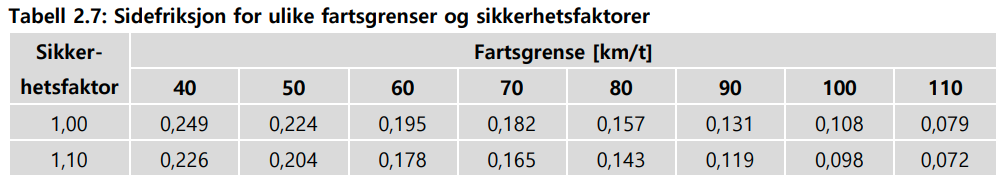
\includegraphics[scale=0.32]{fig/tab2_7}
\end{figure}
\newpage
\op{opgstorlstar2} 
\tagop{
	\# modellering \# areal \# derivasjon
}
Gitt et rektangel med omkrets $ O $, og la $ x $ være den éne sidelengden.
\abc{
	\item  Finn uttrykket til funksjonen $ A(x) $, som viser aralet til rektangelet.
	\item Hvilken form har rektangelet når arealet er størst?
}

\op{opgmagnskal}
\tagop{
	\#logaritmer \#overslag
}
\outl{Momentmagnitudeskalaen} er en skala som brukes til å representere styrken på jordskjelv. Hvis $ S $ er det målte \outl{seismiske momentet} til jordskjelvet, er massemagnituden $ M_w $ gitt som\footnote{Kilde: \net{https://en.wikipedia.org/wiki/Moment_magnitude_scale}{Wikipedia}.}
\[ M_w=\frac{2}{3} \log S-10.7 \]
Energien som jordskjelvet utløser er tilnærmet proporsjonal med $ S $.\os

Gitt to jordskjelv, jordskjelv $ A $ og jordskjelv $ B $, med henholdsvis seismisk moment $ S_A $ og $ S_B $. Si videre at proporsjonalitetskonstanten for energi utløst av det seismiske momentet er likt for begge jordskjelvene. Hvis jordskjelv $ A $ er målt til 1 mer enn jordskjelv $ B $ på momentmagnitudeskalaen, hva er da forholdet mellom energi utløst av jordskjelv $ A $ og energi utløst av jordskjelv $ B $? 
\newpage
\op{opgkast}
Du skal prøve å kaste en ball så langt som mulig langs et flatt strekke. Posisjonen ballen har idét den forlater handen din setter du til $ (0, 0) $. Ved å anta at tyngdekraften deretter er den eneste kraften som virker på ballen, er posisjonen til ballen godt tilnærmet ved uttrykket
\[ \vec{p}_g(t)=\vec{v}t-[0, 5t^2] \]
hvor $ \vec{v}=[v_0 \cos \theta, v_0 \sin \theta] $ er hastighetsvektoren til ballen idét den forlot handen, og $ t $ er antall tidsenheter etter at ballen har forlatt handen. Idét ballen forlater handen din har den farten $ v_0 $, $ \vec{v} $ danner vinkelen $ \theta $ med horisontallinjen.\vsk 

Ut ifra $ \vec{p}_g $, hvilken verdi må $ \theta $ ha for at kastet skal bli lengst mulig?

\op{opgveiformel}
\tagop{
	\# integrasjon \# derivasjon
}
La funksjonen $ s(t) $ beskrive hvor langt et objekt har bevegd seg etter tiden $ t $. Hvi objektet har konstant akselerasjon $ a $, har vi at
\[ s''(t)=a \] 
\abc{
	\item Integrer $ s''(t) $ to ganger slik at du ender opp med et uttrykk for $ s(t) $.
	\item Bestem uttrykkene for $ s(t) $ og $ s'(t) $ når du vet at $ s(t)=0 $ og $ s'(t)=v_0 $.
	\item Hvilken fysisk størrelse representerer $ s'(t) $?
	\item Undersøk begrepet ''bevegelsesligninger''\footnote{''Eqautions of motion på engelsk.} (også kalt ''veiformler'') i en fysikkbok eller på internett. Sammenlign uttrykkene du finner med uttrykket du fant for $ s(t) $. 
}
\newpage
\op{opgbane}
\tagop{
	\#vektorer i planet \#derivasjon
}
Posisjonen $ \vec{s} $ til et objekt som beveger seg i en sirkelbane kan uttrykkes som 
\[ \vec{s} = r[\cos\left(2\pi f t\right), \sin\left(2\pi f t\right)] \]
hvor $ r $ er radien til sirkelbanen, $ t $ er tiden og $ f $ er frekvensen. 
\abc{
	\item $ f $ beskriver antall runder objektet fullfører per tidsenhet\footnote{Hvis tidsenheten er 'sekund', har $ f $ benevningen '1/sekund'.}. Forklar hvorfor $ 2\pi f $ kalles \outl{vinkelfarten} til objektet.
	\item Finn $ \vec{s}\,'(t) $. 
	\item Hva er vinkelen mellom $ \vec{s}(t) $ og $ \vec{s}\,'(t) $?
	\item Bestem lengden til $ \vec{s}\,'(t) $
	\item Finn $ \vec{s}\,''(t) $.
	\item Bestem lengden til $ \vec{s}\,''(t) $
	\item  Hva er vinkelen mellom $ \vec{s}(t) $ og $ \vec{s}\,''(t) $? Peker $ \vec{s}\,''(t) $ innover i sirkelbanen eller ut fra sirkelbanen?
	\item Bruk en fysikkbok eller internett til å undersøke begrepet \outl{sentripetalakselerasjon}. Sammenlign funnene dine i denne oppgaven med informasjonen du finner.
}

\newpage
\op{opgfloogfjere}
\tagop{\# trigonometri}
En tilnærming for høy- og lavvann i Molde er gitt ved \\funksjonen 
\[ f(x)=128+80\cos\left(\frac{3\pi}{37}x\right) \]
hvor $ f $ angir cm over sjøkartnull\footnote{Sjøkartnull er som regel satt til den laveste vannstanden som kan oppnås ut ifra astronomiske betingelser (flo og fjære er i stor grad betinget av hvordan jorda, sola og månen står i forhold til hverandre).} $ t $ timer etter et gitt referanse-tidspunkt. Referansetidspunktet er valgt slik at det ved $ {t=0} $ var høyvann (flo). \os
\abc{
	\item Hva er vannstanden i Molde når det er lavvann (fjøre)?\os
	\item Hvor lang tid er det mellom flo og fjøre? 
}
\mers{Denne oppgaven kan med fordel løses uten digitale hjelpemidler.}


\section{Praktiske oppgaver}
\subsection*{Oppgaver for grunnskole og P-fagene}
\st{Se også oppgaver på \net{https://www.mattelist.no/}{mattelist.no}}

\op{opgrab}
\tagop{\#prosentregning}
Bruk internett til å finne fem varer hvor du har oppgitt følgende:
\begin{itemize}
	\item En original pris og en prosentvis rabatt av denne prisen.
	\item Den nye prisen etter at rabatt er trekt ifra.
\end{itemize}
Undersøk om den nye og den originale prisen samsvarer med rabatten for disse fem varene.

\op{opgstillengde}
Utfør fem stille lengde hopp\footnote{Stille lengde btyr at man skal hoppe med samlede bein, og uten å ta springfart først.}. Finn gjennomstnittslengden og\\ medianlengden for hoppene dine.

\op{opglinjal}
Finn en 20\enh{cm} linjal og og noen små viskelær med lik størrelse. Legg linjalen på et bord slik at 10\enh{cm} av linjalen ligger utenfor kanten av bordet.
\abc{
\item Legg et viskelær på linjalmerket for 5\enh{cm}. Hvor langt ut på linjalen kan du plassere et annet viskelær før linjalen bikker over kanten?  
\item Stable 2 viskelær på linjalmerket for 5\enh{cm}. Hvor langt ut på linjalen kan du plassere et annet viskelær før linjalen bikker over kanten?  
\item Stable 8 viskelær på linjalmerket for 2\enh{cm}. Hvor langt ut på linjalen kan du plassere et annet viskelær før linjalen bikker over kanten? Prøv å svare på spørsmålet før du sjekker svaret i praksis.
}
\newpage
\op{opgstignvater}
\tagop{
\#prosent \#geometri \#algebra \#gjennomsnitt
}
\abc{
\item Beskriv en metode for hvordan du ved hjelp av en vater og et målband/linjal kan bestemme stigningen på et strekke i en bakke.
}
For en bakke som har jevn stigning kan man anslå stigningen på følgende måte
\begin{enumerate}
	\item Lag et merke 5 meter nedenfor et annet merke i bakken. (De 5 metrene måles langs bakken.)
	\item Mål tiden en fotball bruker på å rulle fra det øverste til det nederste merket. Passs på å la ballen trille uten å gi den ekstra fart ved skubbing.
	\item Regn ut gjennomsnittsfarten til ballen mellom de to \\merkene.
	\item Høgdeforskjellen $ h $ mellom de to merkene kan nå tilnærmes ved formelen
	\[ h= \frac{v^2}{19}\]
	hvor $ v $ er gjennomsnittsfarten fra punkt 3. ganget med 2.
	\item La $ l $ være den horisontale  (vannrette) avstanden mellom de to punktene. Da er
	\[ l=\sqrt{5^2-h^2} \]
	\item Den tilnærmede verdien til stigningen er gitt ved brøken $ \frac{h}{l} $.
\end{enumerate}
\abcs{2}{
\item Forklar formelen for $ l $ fra punkt 5.
\item Finn en bakke og sammenlign resultatene fra metoden med en vater og metoden med en fotball.
}

\newpage
\op{opgmaks}
\outl{Makspuls} er et mål på hvor mange hjerteslag hjertet maksimalt kan slå i løpet av et minutt. På siden \href{http://www.trening.no/utholdenhet/ny-formel-for-beregning-av-makspuls/}{\color{blue}trening.no} kan man lese dette:\os
\st{''Den tradisjonelle metoden å estimere maksimalpuls er å ta utgangspunkt i 220 og deretter trekke fra alderen.''}

\textbf{a)} Kall ''maksimalpuls'' for $ m $ og ''alder'' for $ a $ og lag en formel for $ m $ ut i fra sitatet over. \os
\textbf{b)} Bruk formelen fra a) til å regne ut makspulsen din.\vsk

På den samme siden kan vi lese at en ny og bedre metode er slik:\os
''Ta din alder og multipliser dette med 0,64. Deretter trekker du dette fra 211.''\os

\textbf{c)} Lag en formel for $ m $ ut ifra sitatet over.\os

\textbf{d)} Bruk formelen fra c) til å regne ut makspulsen din.

\vsk
For å fysisk måle makspulsen din kan du gjøre dette:
\st{
	\begin{enumerate}
		\item Hopp opp og ned i ca. 30 sekunder (så fort og så høyt du greier).
		\item Tell hjerteslag i 15 sekunder umiddelbart etter hoppingen.
	\end{enumerate}
}
\textbf{e)} Kall ''antall hjerteslag i løpet av 15 sekunder'' for $ A $ og lag en formel for $ m $.\os
\textbf{f)} Bruk formelen fra e) til å regne ut makspulsen din.\os
\textbf{g)} Sammenlign resultatene fra b), d) og f).

\newpage

\op{opgstorlkilopris}
I matbutikker er som regel både pris og kilopris oppgitt for en vare. Vekten til varen finner man på forpakningen til varen. Gå i din lokale matbutikk og velg ut fem varer. Sjekk om kiloprisen som butikken oppgir er rett for disse varene.

\op{opgtrapp}
På nettsiden \net{http://www.viivilla.no/}{viivilla.no} får vi vite at dette er formelen for å lage en perfekt trapp:
\st{''2 ganger opptrinn (trinnhøyde) pluss 1 gang inntrinn (trinndybde) bør bli 62 centimeter (med et slingringsmonn på et par centimeter).''}
\textbf{a)} Kall ''trinnhøyden'' for $ h $ og ''trinndybden'' for $ d $ og skriv opp formelen i sitatet (uten slingringsmonn).\os
\textbf{b)} Sjekk trappene på skolen/i huset ditt, er formelen oppfylt eller ikke?\os

\textbf{c)} Hvis ikke: Hva måtte trinnhøyden vært for at formelen skulle blitt oppfylt?\os

\textbf{d)} Skriv om formelen til en formel for $ h $.

\newpage
\subsection*{Oppgaver for 1T, R1 og R2}
\op{sprint}
\tagop{\#regresjon \#derivasjon \# funksjonsdrøfting}
\begin{itemize}
	\item Sett opp 11 kjegler med 10 meters avstand. 
	\item Ta video av at du springer 100-meteren så fort du kan. 
	\item Bruk videoen og regresjon til å finne en funksjon som gir en god beskrivelse av 100-meteren din. 
	\item Hva var gjennomsnittsfarten din?
	\item Hva var toppfarten din?
	\item På hvilket tidspunkt hadde du størst akselerasjon?
\end{itemize}

\op{friksjonsvinkel}
\tagop{\#trigonometri}
Sett en gjenstand på enden av en planke, og vipp enden varsomt oppover fram til gjenstanden starter å renne nedover planken. Vinkelen hvor bevegelsen starter kalles \outl{friksjonsvinkelen}. Finn friksjonsvinkelen for tre forskjellige gjenstander. Undersøk om friksjonsvinkelen endres hvis gjenstandene og/eller planken vætes. Friksjonsvinkelen skal du finne bare ved å måle hvor høyt planken er vippet, og lengden til planken.


\op{finnvolumvedintegrasjon}
\tagop{\#integrasjon \#regresjon \#omdreiningslegemer}
Finn forskjellige gjenstander det går an å helle vann i. Bruk regresjon og teorien om omdreiningslegemer til å finne en tilnærming for volumet til gjenstanden. Undersøk hvor godt tilnærmingen svarer til virkeligheten.


\newpage
\section{Eksamensoppgaver}
\st{
\eksbm
}

\eksop{GE22}{geks22opg5}
\tagop{
\#regning \#omgjøring av enheter
}
Snorre skal kjøpe ny mobiltelefon.
Ved betaling får han to alternativer:
\begin{itemize}
	\item Alternativ 1: Betal 12 000 kr med en gang
	\item Alternativ 2: Betal 550 kr per måned i to år.
\end{itemize}
Snorre velger alternativ 2. \os

Hvor mye dyrere blir mobiltelefonen med \textsl{alternativ 2} enn med \textsl{alternativ 1}?

\eksop{GV21D1}{GV21D1opg2}
\tagop{
\#regnerekkefølge \#potenser
}
Regn ut $ 3(2+5)-3^2  $

\eksop{GV21D1}{GV21D1opg3}
\tagop{
	\# pi \#rottuttrykk \#desimaltall \#brøk
}
Sorter tallene fra størst til minst
\[ 3,1\qquad\sqrt{9}\qquad2,9\qquad\pi \qquad \frac{32}{10} \]

\newpage
\eksop{GV21D1}{GV21D1opg6}
\tagop{
\#kobinasjonsregning \#logikk
}
Det er 29 bokstaver i alfabetet vårt, og tallsystemet vi vanligvis bruker, har 10 siffer.
Du skal lage en kode med seks tegn. De to første skal være bokstaver, og de fire neste skal være
siffer. En slik kode kan for eksempel være YA6505. \os

Hvilket av tallene under gir antall ulike koder det er mulig å lage? \os
\abch{
\item 290
\item 2320
\item 4\,092\,480
\item 8\,410\,000
}

\eksop{GV21D1}{GV21D1opg9}
\tagop{
\#ligninger \#formler
}
Sett $ n=120 $, og bestem verdien av $ p $ i formelen nedenfor. 
\[ n = 12p + 48 \]

\eksop{GV21D1}{GV21D1opg1} 
\tagop{
\#enheter \#regning
}
En løpebane på en friidrettsbane er 400 meter.
Cornelia løper 6 runder. Hvor langt løper Cornelia? \os

\mers{I eksamenssettet er dette den første av to deloppgaver. Den andre deloppgaven er altså utelatt her.}

\eksop{1PV22D1}{1PV22D1opg5}
\tagop{
\#programmering \#prosentregning
}
\python{python/1pv22d1opg5.py}
En elev har skrevet programkoden ovenfor.
Hva ønsker eleven å finne ut?
Forklar hva som skjer når programmet kjøres.
\newpage
\eksop{1PV22D1}{1PV22D1opg2}
\tagop{\#prosentregning \#statistikk \#tallforståelse}
\fig{1pv22d1opg2}	
Diagrammet viser antall elever ved en videregående skole de fire siste årene.\os

Når var det størst prosentvis økning i antall elever fra et år til det neste?
	
\eksop{1PV23D1}{1PV23D1opg2}
\tagop{\#standardform}
Tall fra FN viser at folketallet på jorda nå har passert 8 milliarder.\os
Forskere har kommet fram til at det er omtrent 2,5 millioner ganger så mange maur som mennesker på jorda.\os

Omtrent hvor mange maur er det på jorden? Skriv svaret\\ på standardform.

\eksop{1PV23D1}{1PV23D1opg3} \vs
\abc{
\item Gi et eksempel på en praktisk situasjon der to størrelser er proporsjonale.
Grunngi at størrelsene er \\proporsjonale.
Tegn en graf som viser sammenhengen mellom størrelsene.
\item Gi et eksempel på en praktisk situasjon der to størrelser er omvendt proporsjonale.
Grunngi at størrelsene er omvendt proporsjonale.
Tegn en graf som viser sammenhengen mellom størrelsene.
}

\newpage
\eksop{1PH23D1}{1PH23D1opg4}
Hunder utvikler seg raskere enn mennesker. Når en hund er 1 år gammel, tilsvarer
det 16 menneskeår. Se tabellen nedenfor.
\begin{figure}
\centering
\includegraphics[scale=0.4]{\figp{1ph23d1opg4}}
\end{figure}
Sondre har en hund som er 2 år gammel. Han mener funksjonen gitt ved
kan brukes som en modell for hvor mange menneskeår en stor hund er når den
er hundeår.
\abc{
\item Forklar hvordan Sondre kan ha kommet fram til dette uttrykket, og argumenter for når modellen er gyldig.
}
Sondre påstår at modellen han har funnet, viser at alderen til en hund er proporsjonal med alderen til et menneske.
\abcs{2}{
\item Stemmer påstanden til Sondre? \\
Husk å argumentere for svaret ditt.
}

\newpage
\eksop{1PH23D1}{1PH23D1opg5}
På en nettside har Dennis funnet teksten nedenfor. \os
\st{
Verdifallet utgjør bilens største kostnad.\os
Verdifallet er i de aller fleste tilfellene størst det første året.\os
For en ny bil kan du vente et verdifall på 20\% det første året.
Deretter 14\% av bruktprisen det andre året, 13\% det tredje året, osv.,
synkende til 10\% det sjette året. \os

Fra og med det sjette året må du regne med et verdifall på 10\% årlig.
}
Dennis vil kjøpe en ny bil som koster 490 000 kroner.\os
Sett opp et regnestykke som vil gi bilens verdi etter 2 år.

\newpage
\section{Teoretiske utvidelser}
\op{opgintpi}
\tagop{\#programmering \#lengden til en graf}
Gitt funksjonen
\[ f(x)=\sqrt{1-x^2} \]
\abc{
	\item Finn $ g(x)=f'(x) $.
	\item I \tmto\, er formelen for lengden $ l $ til en graf gitt. Forklar hvilket tall $ l $ representerer når $ f $ og $ g $ er som gitt i denne oppgaven, og $ a=-1 $ og $ b=1 $.
	\item Bruk en numerisk metode til for å finne en tilnærming for $ l $. Drøft på forhånd hvilke hensyn som må tas for å unngå at skriptet feiler ved kjøring.
}
\newpage

\op{opganubevis}
\tagop{\#følger og rekker \#annuitetslån}
Gitt et annuitetslån (se \am)  med lånebeløp $ L_0 $, årlig rente $ r\% $, og nedbetalingstid $ t $. Lånet skal nedbetales med et årlig terminbeløp $ T $. 
\abc{
	\item La $ L_n $ være resterende lånebeløp etter $ n $-te nedbetaling.\\ Forklar hvorfor 
	\[ L_n=(1+p)L_{n-1}-T \]
	hvor $p=\frac{r}{100}$.
	\item Finn en formel for terminbeløpet $ T $, uttrykt ved $ L_0 $, $ t $ og $ p $.
}
Annuitetslån blir ofte forklart med utgangspunnkt i det vi her skal kalle \textit{spareperspektivet} og \textit{realverdiperspektivet}: \os

\st{
	\textbf{Spareperspektivet}\\
	Vi tenker oss at utlåner oppretter en sparekonto med $ r\% $ årlig rente. I $ t $ år tilføres sparekontoen et årlig innskudd $ T $. Dette skal gi samme resultat som hvis $ L_0 $ hadde blitt satt på sparekonto umiddelbart og forrentet i $ t $ år.
} 

\st{
	\textbf{Nåverdiperspektivet} \\
	Året før nedbetalingen starter setter vi som basisår, og vi tenker at kroneverdien har økt, og vil øke, med $ r\% $ hvert år etter basisåret. Summen av realverdiene til alle terminbeløp skal da tilsvare $ L_0 $.
}
\abcs{3}{
	\item Ta utgangspunkt i likningen merket med (*) i løsningsforslaget, og forklar hva de to sidene i likningen beskriver ut ifra spareperspektivet.
	\item Ta utgangspunkt i likningen merket med (*) i løsningsforslaget, og lag en likning som beskriver nåverdiperspektivet.
}
\newpage
\op{utfrskrasjfunk}
\tagop{\#rasjonale funksjoner \#funksjonsdrøfting \#digital graftegning}
Definer funksjonen
\[ \frac{ax-b}{x-c} \]
i en digital graftegner (GeoGebra). Beskriv hva som skjer med grafen til $ f $ når du øker/minker én av $ a $, $ b $ og $ c $ på intervallet $ [-3, 3] $.

\eksop{R1H23D1}{R1H23D1opg4}
Funksjonen $ f $ er gitt ved
\[ f(x)=2x^2-9x-2 \]
Egil ønsker å lage et program som regner ut koordinatane til bunn-punktet på grafen til $ f $. Han har skrevet koden nedenfor.
\pythonut{python/r1h23d1opg4.py}{
	Bunnpunktet er (3, -11)
}
\abc{
	\item Forklar hvilken strategi Egil har brukt.	
}
Svaret han får er ikke rett.
\abcs{2}{
	\item Foreslå en endring i koden som vil gi Egil et riktigere svar.
}
\newpage
\eksop{R1V23D1}{r1v23d1opg4}
En elev har fått følgende oppgave:
\st{
	Funksjonen $ f $ er gitt ved
	\[ f(x)=(x^2-9)^4\qquad,\qquad x\in(0, 3) \]
	Et rektangel $ R $ har hjørne i $ (0, 0) $, $ (t, 0) $, $ (t, f(t)) $ og $ (0, f(t)) $.	\os
	Bestem den verdien av $ t $ som gjør at $ R $ har størst areal.
	\fig{r1v23d1opg4}
}
For å løse oppgaven har eleven lagd følgende program:
\python{python/r1v23d1opg4.py}
\abc{
	\item Forklar strategien eleven har brukt.
	\item Løs oppgaven eleven har fått.
}
\newpage
\eksop{R2V23D1}{r2v23d1opg4}
En elev har skrevet følgende kode:
\python{python/r2v23d1opg4.py}
\abc{
	\item Forklar hva eleven vil regne ut.
	\item Hva blir resultatet når man kjører programmet, hvis N settes til 100 i linje 4?
}


\end{document}

